\documentclass[11pt]{article}
\usepackage{latexsym}
\usepackage{natbib}
\usepackage{graphicx}
\usepackage{caption}
\usepackage{subcaption}
\usepackage{listings}
\usepackage{algorithm}
\usepackage{algpseudocode}

\title{Homework 5: Reinforcement Learning}
\author{Shun Zhang}
\date{}

\begin{document}
\maketitle

\section{Q-Learning}

$$Q(s, a) = (1 - \alpha) Q(s, a) + \alpha (r + \gamma Q(s', a'))$$

$$correction = r + \gamma Q(s', a') - Q(s, a)$$
$$w_i = w_i + \alpha [correction] f_i(s, a)$$

\begin{figure}[h]
\centering
\begin{subfigure}{0.9\textwidth}
	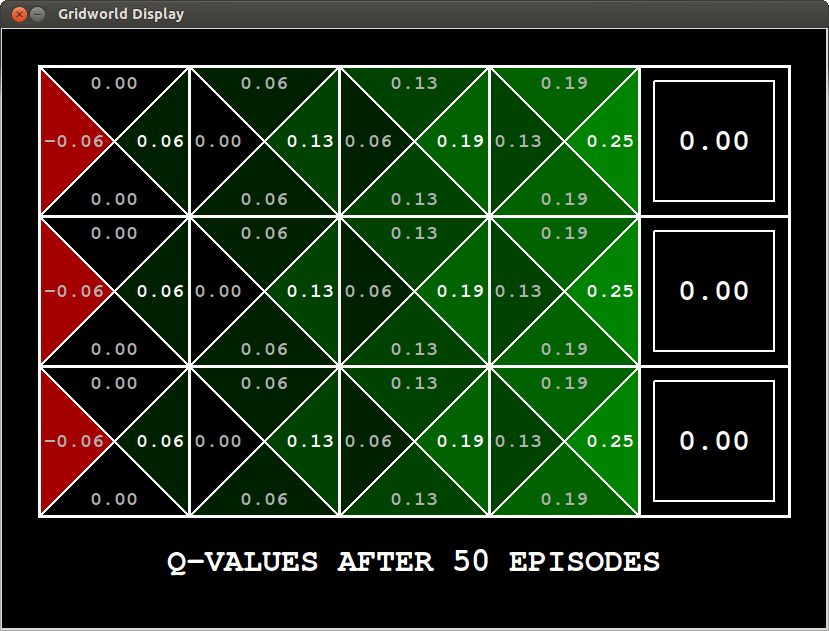
\includegraphics[width=\textwidth]{figure/sidewalk}
\end{subfigure}
\begin{subfigure}{0.9\textwidth}
	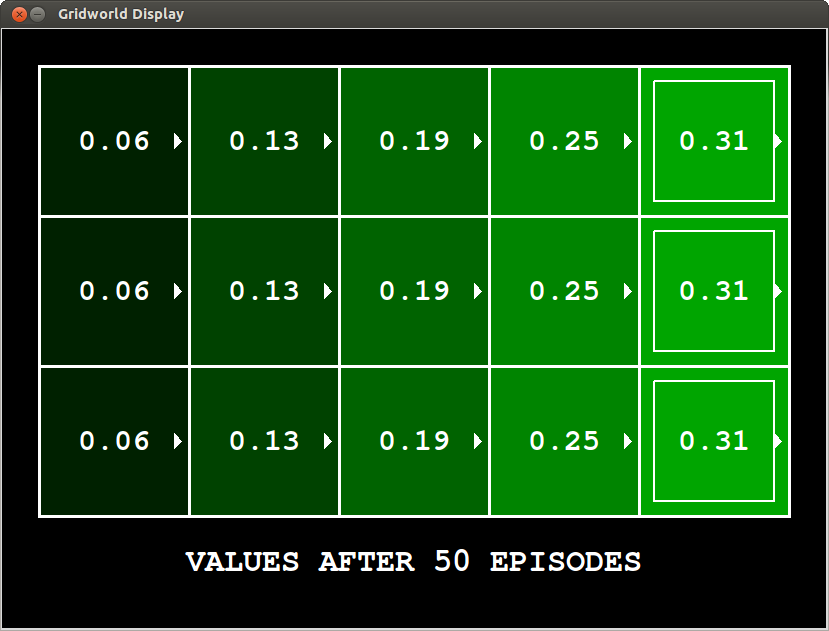
\includegraphics[width=\textwidth]{figure/sidewalk_v}
\end{subfigure}
\label{fig:rep}
\end{figure}

\begin{figure}[h]
\centering
\begin{subfigure}{0.49\textwidth}
	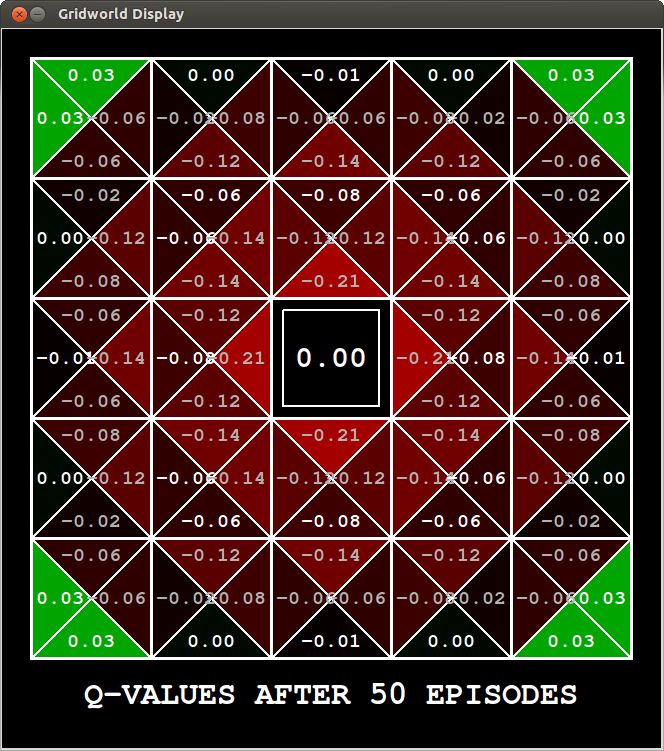
\includegraphics[width=\textwidth]{figure/obstacle}
\end{subfigure}
\begin{subfigure}{0.49\textwidth}
	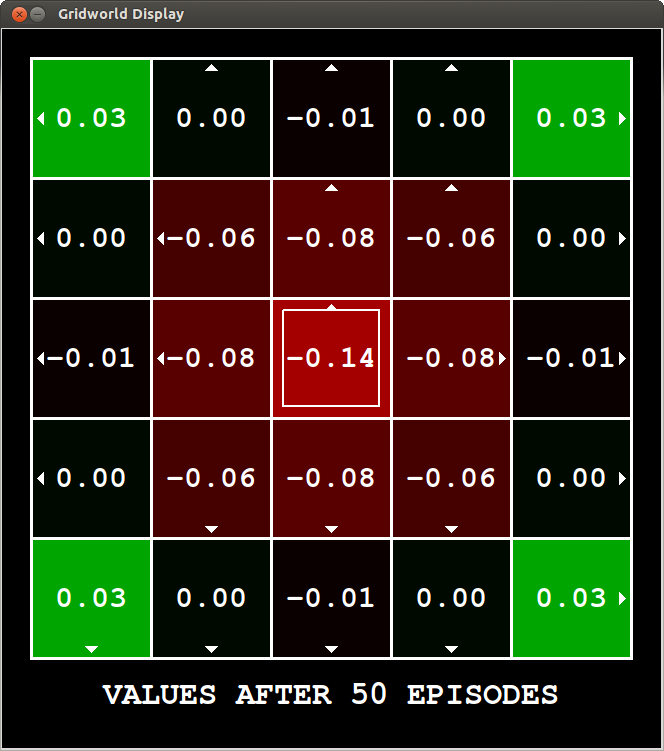
\includegraphics[width=\textwidth]{figure/obstacle_policy}
\end{subfigure}
\label{fig:rep}
\end{figure}

\begin{figure}[h]
\centering
\begin{subfigure}{0.9\textwidth}
	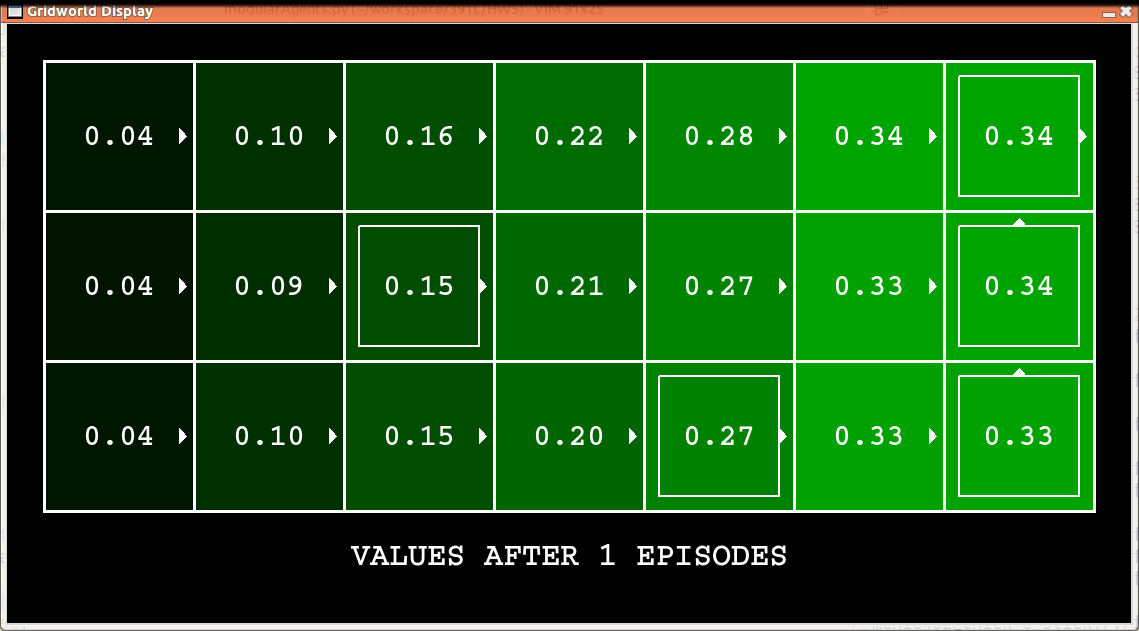
\includegraphics[width=\textwidth]{figure/hybird_walk}
\end{subfigure}
\begin{subfigure}{0.9\textwidth}
	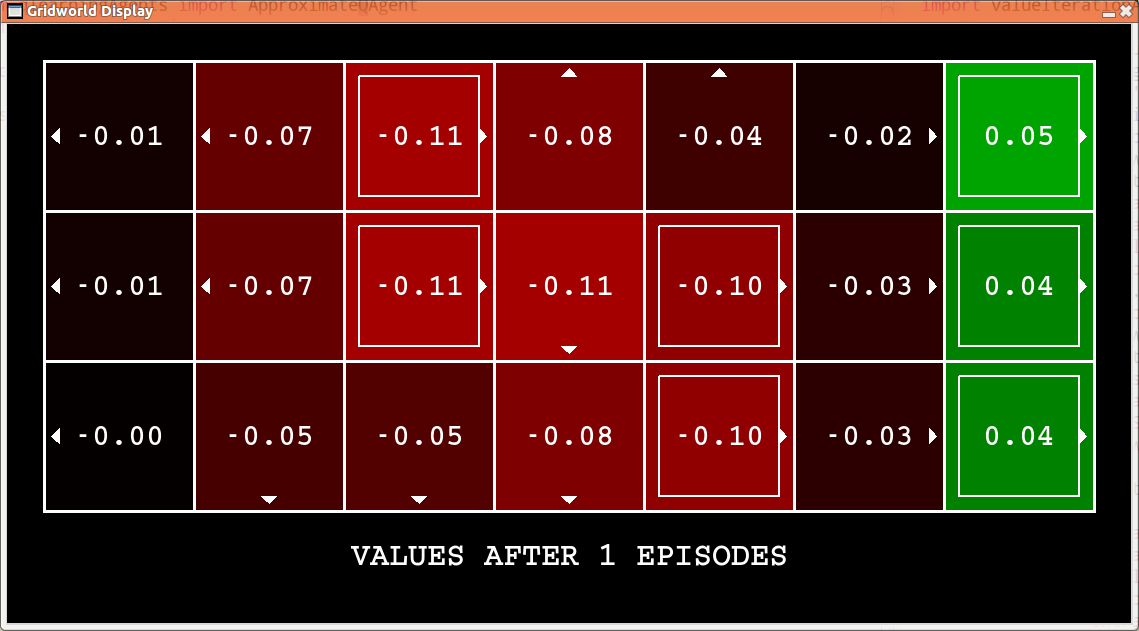
\includegraphics[width=\textwidth]{figure/hybird_obstacle}
\end{subfigure}
\label{fig:rep}
\end{figure}

\end{document}
